\documentclass[tikz,border=5mm]{standalone}
\usepackage{pgfplots}
\usepackage{amsmath}
\pgfplotsset{compat=1.18}

\definecolor{vecred}{RGB}{230, 0, 0}
\definecolor{vecblue}{RGB}{0, 0, 230}
\definecolor{vecgreen}{RGB}{0, 130, 0}

\begin{document}
	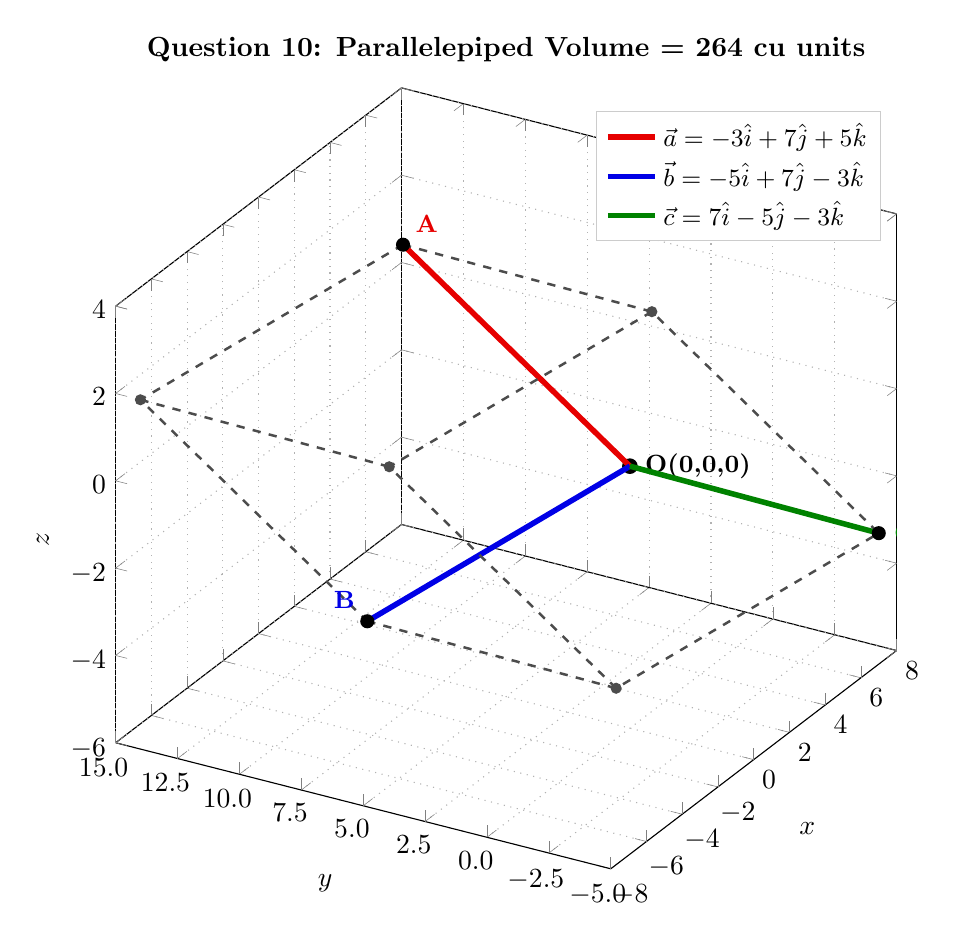
\begin{tikzpicture}
		\begin{axis}[
			width=11.5cm, height=11.5cm,
			view={-60}{30},
			title={\textbf{Question 10: Parallelepiped Volume = 264 cu units}},
			xlabel={$x$}, ylabel={$y$}, zlabel={$z$},
			xmin=-8, xmax=8,
			ymin=-5, ymax=15,
			zmin=-6, zmax=4,
			xtick={-8, -6, -4, -2, 0, 2, 4, 6, 8},
			ytick={-5.0, -2.5, 0.0, 2.5, 5.0, 7.5, 10.0, 12.5, 15.0},
			yticklabel style={/pgf/number format/fixed, /pgf/number format/precision=1, /pgf/number format/zerofill},
			ztick={-6, -4, -2, 0, 2, 4},
			grid=both,
			grid style={dotted, gray!60},
			legend cell align={left},
			legend style={at={(0.98,0.97)}, anchor=north east, font=\small, draw=gray!40}
			]
			% Origin O(0,0,0)
			\node[circle, fill=black, inner sep=2pt] at (axis cs:0,0,0) {};
			\node[right=2pt, font=\bfseries\small] at (axis cs:0,0,0) {O(0,0,0)};
			
			% Vector a = -3i + 7j + 5k
			\addplot3[vecred, line width=2pt] coordinates {(0,0,0) (-3,7,5)};
			\addlegendentry{$\vec{a} = -3\hat{i} + 7\hat{j} + 5\hat{k}$}
			
			% Vector b = -5i + 7j - 3k
			\addplot3[vecblue, line width=2pt] coordinates {(0,0,0) (-5,7,-3)};
			\addlegendentry{$\vec{b} = -5\hat{i} + 7\hat{j} - 3\hat{k}$}
			
			% Vector c = 7i - 5j - 3k
			\addplot3[vecgreen, line width=2pt] coordinates {(0,0,0) (7,-5,-3)};
			\addlegendentry{$\vec{c} = 7\hat{i} - 5\hat{j} - 3\hat{k}$}
			
			% Parallelepiped dashed edges
			\addplot3[gray!60!black, dashed, line width=0.9pt] coordinates {(-3,7,5) (-8,14,2) (-5,7,-3)};
			\addplot3[gray!60!black, dashed, line width=0.9pt] coordinates {(-3,7,5) (4,2,2) (7,-5,-3)};
			\addplot3[gray!60!black, dashed, line width=0.9pt] coordinates {(-5,7,-3) (2,2,-6) (7,-5,-3)};
			\addplot3[gray!60!black, dashed, line width=0.9pt] coordinates {(-8,14,2) (-1,9,-1)};
			\addplot3[gray!60!black, dashed, line width=0.9pt] coordinates {(4,2,2) (-1,9,-1)};
			\addplot3[gray!60!black, dashed, line width=0.9pt] coordinates {(2,2,-6) (-1,9,-1)};
			
			% Vertices and labels
			\node[circle, fill=black, inner sep=1.8pt] at (axis cs:-3,7,5) {};
			\node[above right=1pt, font=\bfseries\small, text=vecred] at (axis cs:-3,7,5) {A};
			
			\node[circle, fill=black, inner sep=1.8pt] at (axis cs:-5,7,-3) {};
			\node[above left=1pt, font=\bfseries\small, text=vecblue] at (axis cs:-5,7,-3) {B};
			
			\node[circle, fill=black, inner sep=1.8pt] at (axis cs:7,-5,-3) {};
			\node[right=2pt, font=\bfseries\small, text=vecgreen] at (axis cs:7,-5,-3) {C};
			
			\addplot3[only marks, mark=*, mark size=1.8pt, gray!60!black] coordinates {
				(-8,14,2) (4,2,2) (2,2,-6) (-1,9,-1)
			};
		\end{axis}
	\end{tikzpicture}
\end{document}